\documentclass[en]{../../../eplsummary}

\usepackage{listings}

\hypertitle{constraint-INGI2365}{8}{INGI}{2365}
{Houtain Nicolas}
{Yves Deville}
$$$$

\section{Constraint Programming (CP)}
\textsc{CP = Model + Search}

\begin{enumerate} 
    \item \textsc{Model} : Describe real world problem with
        \begin{itemize}
            \item \textbf{Variables} : $X = \{x_1, x_2,\cdots, x_n\}$
            \item \textbf{Domains} : $D = \{ D(x_1), D(x_2),\cdots,
                D(x_n)\}$

                \begin{itemize}
                    \item[Ex:] Booleans, \textbf{finite domains}, finite
                        set, intervals, continuous domains,\ldots
                \end{itemize}
            \item \textbf{Constraints} : $C = \{c_1, c_2,\cdots, C_e\}$
                \begin{itemize}
                    \item A \textbf{scope} $scp(c) = (x_1, x_2,\cdots,x_r)$ : is the
                        variables constrained by c.
                    \item A \textbf{relation} $rel(c)$ : value combinations accepted by
                        c
                \end{itemize}
            \item \textbf{Objective function} : $O = solution \to \R$
        \end{itemize}

        \paragraph{Types}
        \begin{enumerate}
            \item CSP = (X, D, C)
            \item COP = (X, D, C, O)
        \end{enumerate}

        \paragraph{Declarative} : describe what you want not how to get it
    \item[+]
    \item \textsc{Search} : Describe how to solve the problem.
        \begin{itemize}
            \item \textbf{Propagation} : Use constraints to remove
                \textit{useless} (doesn't remove solution) parts of the search space
                \begin{center}
                    \scriptsize
                    \textit{Need choice between more pruning with more
                        expensive to compute or less proning cheaper to
                    compute}
                \end{center}

                \begin{itemize}
                    \item Consistencies : Require that all the values
                        are able to satisfy their constaints in
                        \textbf{isolation}
                \end{itemize}
            \item \textbf{Backtrackink Tree Search} : Explore search
                space by taking decisions and backtracking (with
                remembering decision)
        \end{itemize}

        \paragraph{Search space} = $D(x_1) \times D(x_2) \times \cdots \times D(x_n)$
\end{enumerate}


\paragraph{Solution}
A solution to a CSP is 
\begin{enumerate}
    \item An assigment of variabels ot values in their domains
    \item Such that all the constraints are respected
\end{enumerate}


% TODO ---v
\subsection{Constraints}
\subsubsection{Auxiliary variables}
Variables used to help/improve modeling

Vs

variable which reprendt the decision CP has to make

reducundant constraint : constraint that does not exclude any previous solution,
improve prining (reduce search space), improve communication
\subsubsection{Global constraint}
\subsection{Symmetry}


\section{Propagation}
\begin{itemize}
    \item $n$ variables
    \item domains of size $d$
    \item $e constraints$
    \item maximum arity $r$
\end{itemize}

\subsection{Without propagation (Bruteforce)}:

\begin{tabular}{m{6cm}cm{6cm}}
    \begin{itemize}
        \item $O(d^n)$ possible assignements
        \item $O(r)$ to test a constraint
        \item $O(e \times r)$ to test all constraint
    \end{itemize}
    & $\to$ &
    \textbf{Global complexity}: $O(d^n \times e \times r)$
\end{tabular}

\subsection{Fonctionnement}

The goal of propagation is to \textbf{reduce} the search space
(\textit{reduction domains, reduction constraints, addition constraint})
but do not remove solutions.

The propagation is used before the search and all along the search.

\subsubsection{Partial solution} 

A partial instantiation gives values to some variables.
It's a \textbf{partial solution} IFF
\begin{center}
    for all constraint c : if all variables assigned $\to$ c satisfied  
\end{center}


The propagation perfom checking and \textcolor{red}{fail} when there is
no partial solution : checking fails or there is inconsistency (empty domain,\ldots)

\subsubsection{Level of propagation}
\begin{tabular}{ccc}
    \textbf{Weaker} & $\Rightarrow$ & \textbf{Stronger} \\
    Less pruning & & More pruning \\
    Cheaper to compute & & More expensive to compute \\
\end{tabular}


\subsection{Consistency}

\subsubsection{Filtering consistencies}

if $x$ is a domain filtering consistency, a propagator for $x$ will :
from CSP(X, D, X) 
\begin{itemize}
    \item return (X, D', C) such that
        \begin{itemize}
            \item D' $\subseteq$ D
            \item (X, D, C) and (X, D', C) equivalent
            \item D' is a nonempty partial solution
            \item (X, D', C) respect $x$
        \end{itemize}
    \item return \textcolor{red}{fail} if no such CSP exists.

        $\to$ not possible to satisfy consistency = unsatisfiable CSP
\end{itemize}



\subsubsection{Arc consistency (AC)}
Strongest filtering when considering constraints in isolation.

\paragraph{CSP} A \underline{binary} CSP (\textsc{X, D, C}) is AC iff all constraints $c \in C$ are AC

\paragraph{Constraint} A \underline{binary} constraint $c$ on $x, y$ is AC iff
\begin{lstlisting}[mathescape]
    $\forall a \in D(x), \exists b \in D(y) : (a,b) \in c$ 
    $\forall a \in D(x), \exists b \in D(y) : (a,b) \in c$
\end{lstlisting}

$\to$ It means that all the value of variables are \textbf{supported}

\begin{figure}[!h]
\centering
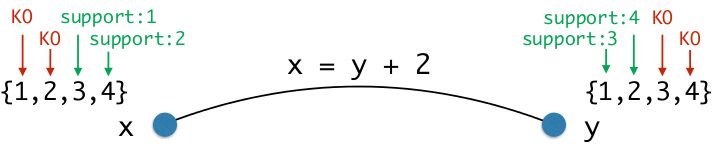
\includegraphics[width=10cm]{img/AC.png}
\caption{AC example}
\end{figure}


\subsubsection{Generalize arc consistency (GAC)}
Strongest filtering when considering constraints in isolation.

\paragraph{CSP} A CSP (\textsc{X, D, C}) is GAC iff all constraints $c \in C$ are GAC

\paragraph{Constraint} A constraint $c$ is GAC iff
\begin{lstlisting}[mathescape]
    $\forall x_i \in scope(c)$
        $\forall a_i \in D(x_i)$
            $\exists a_1,..., a_{i-1}, a_{i+1},..., a_r $
                    $\in D(x_1) \times ... \times D(x_{i-1}) \times D(x_{i+1}) \times ... \times D(x_r)$
                $(a_1,...,a_r) \in c$

\end{lstlisting}

\begin{figure}[!h]
\centering
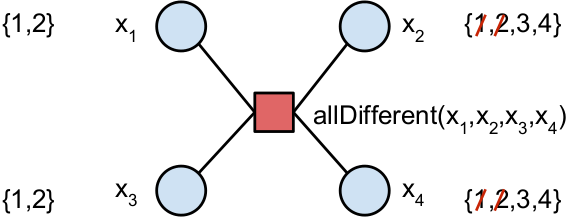
\includegraphics[width=8cm]{img/GAC.png}
\caption{GAC example}
\end{figure}

\subsubsection{Propagation}

If a value is not GAC, it can never be part of solution\ldots So, 
GAC propagation remove all values that are not GAC!

\paragraph{GAC $\neq$ Satisfiability} : A CSP that is GAC may not
be satisfiable


\subsection{Fixed point algorithm}

Fixed point algorithm is use to restrict the domains such that all the 
constraints are GAC.



\subsection{Constraint based propagation}

\subsection{Value based propagation}





\section{Examen questions}

\begin{enumerate}
    \item \begin{itemize}
            \item Formal definition of CSP
            \item Formal definition of COP
            \item Definition of a constraint
            \item Principle of search in CP
            \item Current DOmain
            \item Communication in CP
            \item Computational model
        \end{itemize}
    \item 
    \item \begin{itemize}
            \item Consistency
            \item Definition of GAC
            \item Value based fixed point
            \item (G)AC3, AC3rm, AC2001, (G)AC4, AC6
            \item Complexities
            \item Invariant on their data structure
        \end{itemize}

\end{enumerate}

\end{document}
